% Flowchart of the base GSK algorithm, in the style of the original GSK paper
% (Fig. 10): a clean vertical flow with rounded terminals, plain (unfilled)
% process boxes, a diamond decision, and a loop-back. No background colours.
% Standalone -> fig_gsk_flowchart.pdf.  Compile: pdflatex fig_gsk_flowchart_src.tex.
\documentclass[border=6pt]{standalone}
\usepackage{tikz}
\usepackage{amsmath}
\usetikzlibrary{shapes.geometric, arrows.meta, positioning, calc}
\begin{document}
\hyphenpenalty=10000\exhyphenpenalty=10000\relax
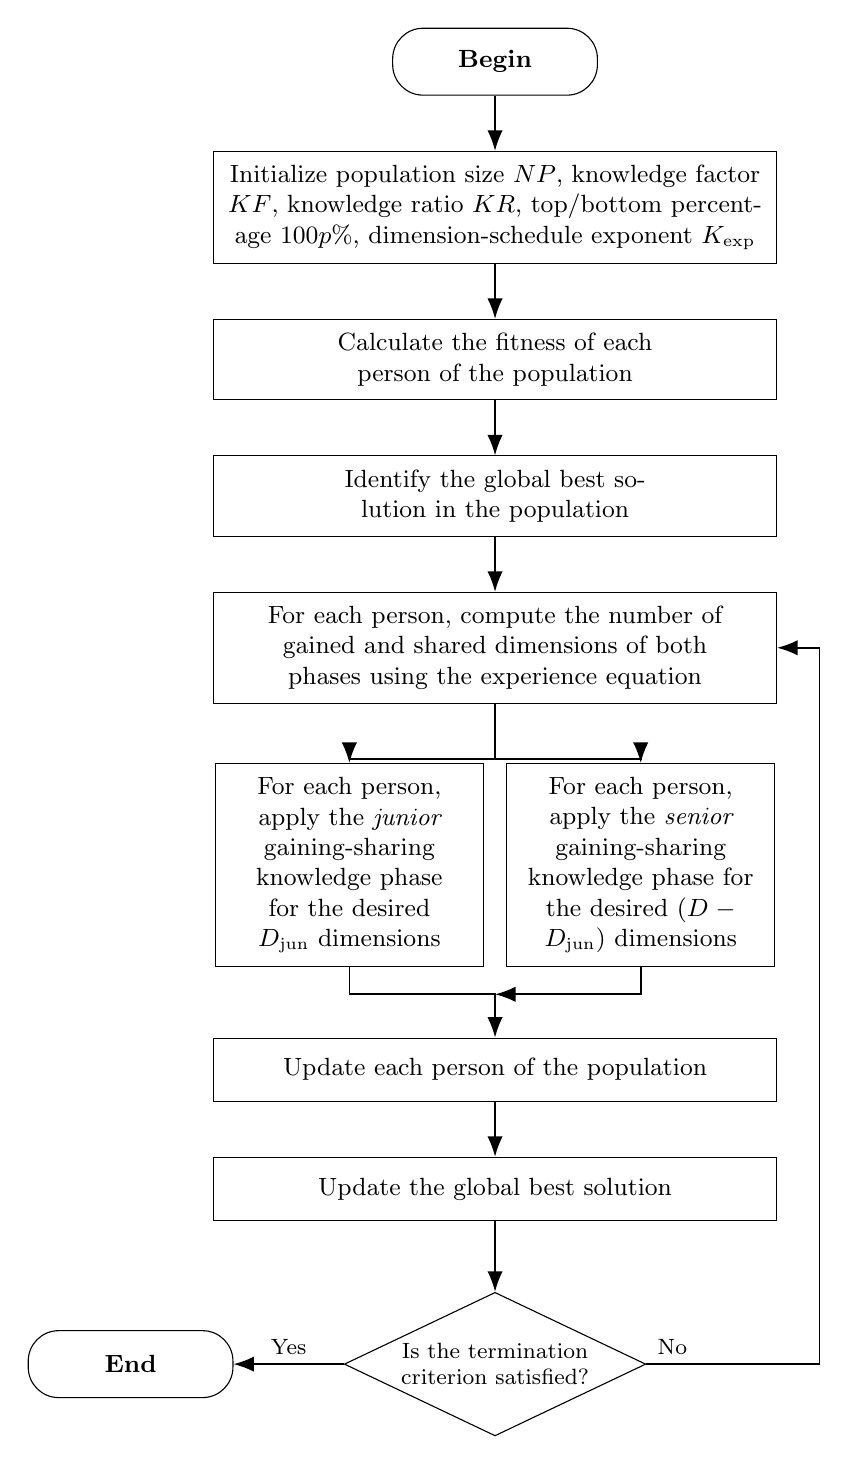
\begin{tikzpicture}[
  font=\small,
  node distance=7mm,
  term/.style={rectangle, rounded corners=11pt, draw=black, fill=white,
               minimum width=2.6cm, minimum height=0.85cm, align=center},
  proc/.style={rectangle, draw=black, fill=white, text width=6.8cm,
               minimum height=0.8cm, align=center, inner sep=5pt},
  half/.style={rectangle, draw=black, fill=white, text width=3.05cm,
               minimum height=1.5cm, align=center, inner sep=5pt},
  dec/.style={diamond, aspect=2.1, draw=black, fill=white, align=center,
              inner sep=1pt, text width=2.5cm, font=\footnotesize},
  arr/.style={-{Latex[length=2.6mm]}, semithick},
  lbl/.style={font=\footnotesize},
]
\node (begin) [term] {\textbf{Begin}};
\node (init)  [proc, below=of begin]
  {Initialize population size $NP$, knowledge factor $KF$, knowledge ratio
   $KR$, top/bottom percentage $100p\%$, dimension-schedule exponent $K_{\exp}$};
\node (fit)   [proc, below=of init]
  {Calculate the fitness of each person of the population};
\node (best)  [proc, below=of fit]
  {Identify the global best solution in the population};
\node (dims)  [proc, below=of best]
  {For each person, compute the number of gained and shared dimensions of both
   phases using the experience equation};
% junior / senior split (kept well clear of the compute-dimensions box)
\node (junior) [half] at ($(dims.south)+(-1.85cm,-2.05cm)$)
  {For each person, apply the \emph{junior} gaining-sharing knowledge phase for
   the desired $D_{\text{jun}}$ dimensions};
\node (senior) [half] at ($(dims.south)+(1.85cm,-2.05cm)$)
  {For each person, apply the \emph{senior} gaining-sharing knowledge phase for
   the desired $(D-D_{\text{jun}})$ dimensions};
\node (upd)   [proc] at ($(junior.south)!0.5!(senior.south)+(0,-1.3cm)$)
  {Update each person of the population};
\node (gbest) [proc, below=of upd]
  {Update the global best solution};
\node (dec)   [dec, below=9mm of gbest] {Is the termination criterion satisfied?};
\node (end)   [term, left=14mm of dec] {\textbf{End}};
% edges
\draw [arr] (begin) -- (init);
\draw [arr] (init)  -- (fit);
\draw [arr] (fit)   -- (best);
\draw [arr] (best)  -- (dims);
\coordinate (br) at ($(dims.south)+(0,-0.7cm)$);
\draw (dims.south) -- (br);
\draw [arr] (br) -| (junior.north);
\draw [arr] (br) -| (senior.north);
\draw [arr] (junior.south) |- ($(upd.north)+(0,0.55cm)$) -- (upd.north);
\draw [arr] (senior.south) |- ($(upd.north)+(0,0.55cm)$);
\draw [arr] (upd)   -- (gbest);
\draw [arr] (gbest) -- (dec);
\draw [arr] (dec) -- node[lbl,above]{Yes} (end);
% loop-back (No) on the right side, up to the compute-dimensions step
\coordinate (rail) at ($(dec.east)+(2.2cm,0)$);
\draw [arr] (dec.east) -- node[lbl,above,pos=0.15]{No} (rail)
      -- (rail |- dims.east) -- (dims.east);
\end{tikzpicture}
\end{document}
